\begin{task}{4, Integrating a new model}

\paragraph{1. Implementation of the SIR Model into Vadere}

\begin{figure}[H]
\centering
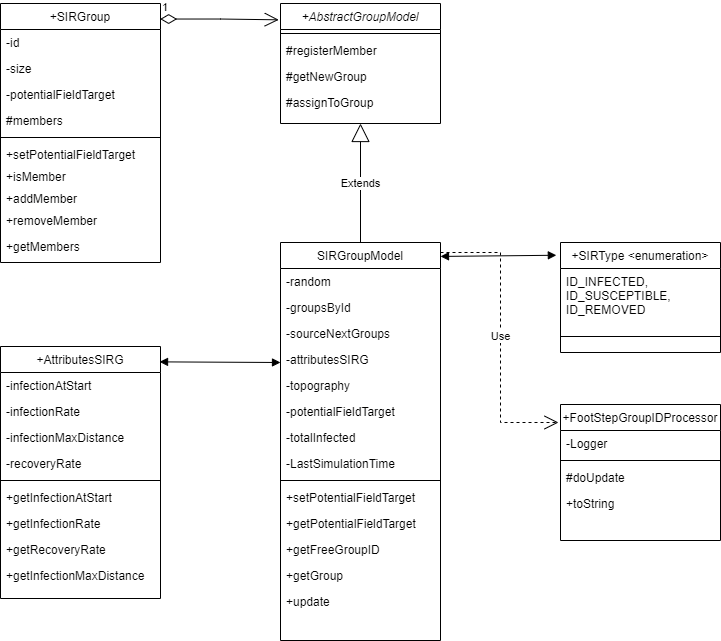
\includegraphics[width=0.7\textwidth]{report-template/images/taask4.1.png}
\caption{UML diagram of SIR Model}
\label{fig:fig4uml}
\end{figure}
The UML diagram above \ref{fig:fig4uml} describes the relationships between the classes \verb+SIRGroupModel+, \verb+SIRGroup+, \verb+AbstractGroupModel+, \verb+AttributeSIRG+, \verb+SIRType+ and \verb+FootStepGroupIDProcessor+. For some classes only important functions were listed.
\begin{description}
    \item \verb+SIRGroupModel+ is the main class for handling the behaviour of groups in the SIR model. It keeps track of the group ids and assigns pedestrian to each of the groups in the SIR model. The update function does most of this work. It implements calculation for infecting and recovering pedestrians and also contains the efficient neighbourhood lookup using LinkedCellsGrid to check for susceptible pedestrians.
    \item \verb+SIRGroup+ contains essential information about a SIR group as well as adding and removing members. Furthermore it defines the type of the generic class \verb+AbstractGroupModel+, which \verb+SIRGroupModel+ inherits from. This leads \verb+SIRGroupModel+ returning groups of type \verb+SIRGroup+ for the inherited functions. 
    \item \verb+AttributesSIRG+ contains the parameters of our SIR model and is saved as attribute in the \verb+SIRGroupModel+. Infection rate and recovery rate can be changed here for example. Additionally the values in this class the initial parameters when loading the SIR model into Vadere and can be changed in the Vadere editor before running a simulation.
    \item \verb+SIRType+ is simple enumeration class which contains 3 different states in the SIR model. This class is used in \verb+SIRGroupModel+ to determine the pedestrian state in the SIR model.
    \item \verb+FootStepProcessor+ uses \verb+SIRGroupModel+ to log information about SIR simulation. This class is an additional output processor that can be linked in the Vadere. When running the SIR model this processor output additional information about the SIR model.
\end{description}

% uml
%\textbf{SirGroupModel}: is the main class which is the extension of the AbstractGroupModel. 
%Group the pedestrains by the ID, and also updating method does the main job of traversing all the pedestrians, checking the infected rate, and determining if the pedestrian is lucky enough to get infected or not. 
%\textbf{SIRgroup}: this class is the aggregation of the AbstractGroupModel, a unique ID for every member, which can be used to manipulate the members to be added, or deleted. 
%\textbf{AttributeSIRG}:  associated with the  SirGroupModel, contains the basic information of infection state, infection rate, and Recovery rate, and the infection maximal distance. 
%\textbf{SIRType} also associated with the SIRgroupModel, store the states of the pedestrian.  \textbf{FootStepGroupIDProcessor} one additional class used by the SirGroupModel, outputs the processor and saves the result as a file. the doUpdate method is the most important, every step will update new info on the current time step, pedestrian, and group. 

\paragraph{2. Description of the output processor}
In this part we use our own output processor \verb+SecondGroupIDProcessor+ instead of \verb+FootStepGroupIDProcessor+, which can be found in the same folder as the other output processors. This class simply writes down at each time-step the pedestrian id and group id of the pedestrian. This way even pedestrians that did not move are tracked unlike in the footstep processor and this allows for a more direct output. Of course we could have set up a program to read the footstep processor output and memorize the group ID from the previous time-step if the next time-step does not include a pedestrian but this did not occur to us at the time.

In the visualization we use a python notebook that loads the file and extracts the group IDs in each time-step and then plots percentages of the group IDs. This is handled in the python notebook \verb+visualizeSIR.ipynb+ which generates graphs tracking changes of the SIR groups. \textit{Note that for task 4 and task 5 the vadere project with its scenarios are placed in the folder} \verb+Exercise-2\vadere-project-tas45+.

\paragraph{3. SIR group visualization}
To color the pedestrians based on their group we need to put the group id and its corresponding color into the \verb+colorMap+ in the class \verb+SimulationModel.java+. We assigned the following colors to each group id:
\begin{itemize}
    \item 0 = Red
    \item 1 = Black
    \item 2 = Blue
\end{itemize}
We also didn't use green or white for susceptible individuals, because the pedestrian spawning area is visualized with green and the background color is white. To visualize the pedestrians according to group color during simulation we need to set the \verb+DefaultSimulationConfig.agentColoring = AgentColoring.GROUP+. It is noteworthy that due to our own implementation of the output processor in \verb+SecondGroupIDProcessor+ we have only implemented the visualization of groups during simulation. Visualization of groups in post-visualization is not supported in this iteration of our code.

\paragraph{4. Using LinkedCellsGrid to improve efficiency} To increase the efficiency of finding nearby pedestrians we modified the \verb+update(...)+ function in \verb+SIRGroupModel.java+. To get the neighbourhood of given radius more efficiently the LinkedCellsGrid slices the 2 dimensional space into uniform squares of given side length. It then only checks the squares which are less than the radius of the neighbourhood away from a given position's square.

\paragraph{5.1 Test: comparing infection rates}
% Tested+visualized scenario in figure 6, left, without recovered state?
% How long does it take for half of the population to be infected?
% Increase the infectionRate of the model using the GUI, and run the previous test again. Plot both results in one graph. How long does it take to infect half the population now?
In this test we setup a large area in which we randomly placed a 1000 pedestrians uniformly distributed. In this test we want to compare how fast 50\% of the pedestrians become infected depending on the infection rates. We have setup the same starting amount of $10$ infected pedestrians in both scenarios. In this test we only changed \verb+infectionRate+, but a full list will be provided at the end of this section. Running the tests yields the following results, where the \verb+infectionRate+ is the probability for and the time is how long it takes until 50\% of the pedestrians are infected:
\begin{center}
\begin{tabular}{ |c|c|c| } 
 \hline
& Scenario (a) & Scenario (b) \\
\hline
\verb+infectionRate+ & $0.01$ & $0.05$ \\
\hline
time (in seconds) & $36.2$ & $4$\\
\hline
\end{tabular}
\end{center}
We see that with $5$ times the infection rate the time until 50\% of the pedestrians are infected decreases from $36.2$ seconds to $4$ seconds. We know from the mathematical nature of infection spreading that it has an exponential behaviour. Hence the immense decrease in time until 50\% is infected is expected. In the figures \ref{fig:fig6sim} below we see the results after running both simulations. Further more in figure \ref{fig:fig6sim}(c) we see a graph comparing the infection spread between both scenarios.
\begin{figure}[H]
\centering
\subfigure[infection rate 0.01 at second 36.2]{
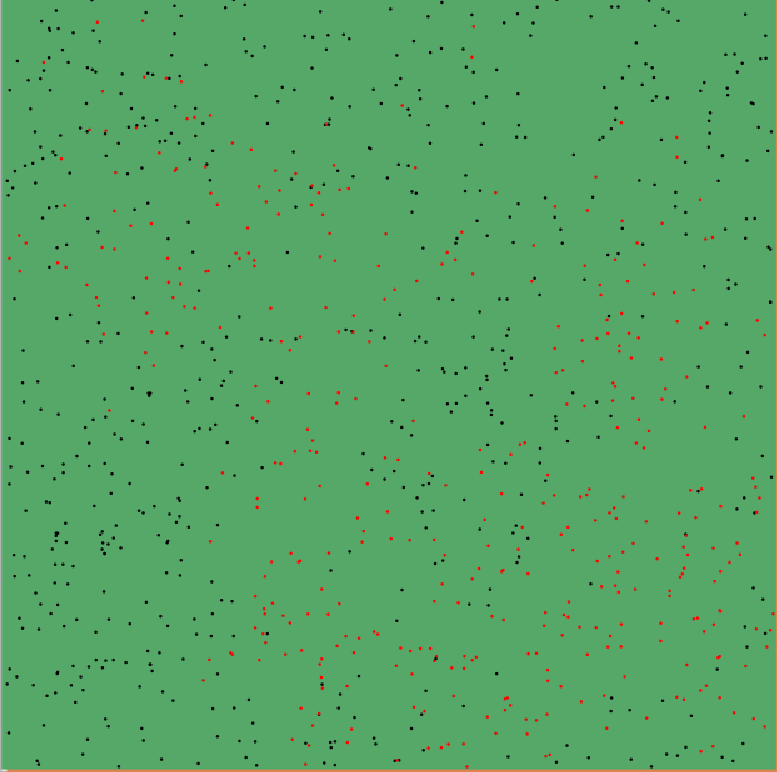
\includegraphics[width=0.4\textwidth]{report-template/images/001_no_recovery_16_2.png}}
\subfigure[infection rate 0.05 at second 4]{
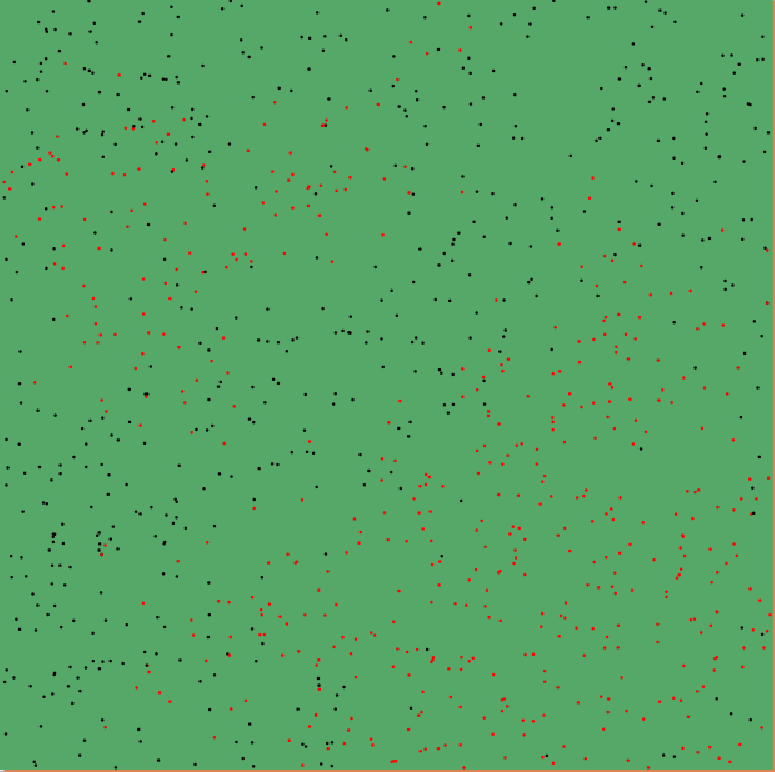
\includegraphics[width=0.4\textwidth]{report-template/images/005_no_recovery_4_0.png}}
\subfigure[Comparison between different spread rates]{
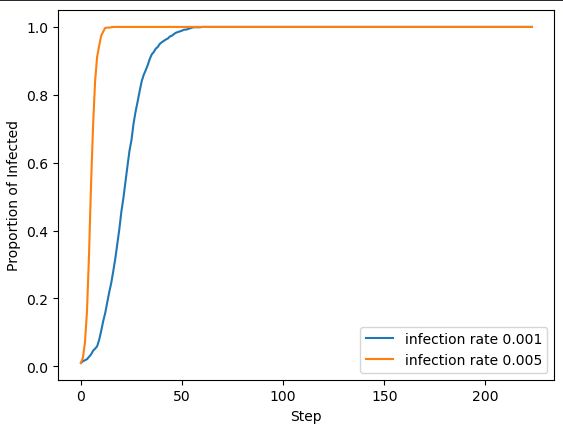
\includegraphics[width=0.5\textwidth]{report-template/images/rateplot.png}}
\caption{Comparison of the figure 6 simulations}
\label{fig:fig6sim}
\end{figure}

\noindent Scenario \ref{fig:fig6sim}(a) parameters
\begin{verbatim}
"infectionsAtStart" : 10,
"infectionRate" : 0.01,
"infectionMaxDistance" : 10.0,
"recoveryRate" : 0.0
"infectionRateWhenAdded" : 0.0
\end{verbatim}
Scenario \ref{fig:fig6sim}(b) parameters
\begin{verbatim}
"infectionsAtStart" : 10,
"infectionRate" : 0.05,
"infectionMaxDistance" : 10.0,
"recoveryRate" : 0.0
"infectionRateWhenAdded" : 0.0
\end{verbatim}

\paragraph{5.2 Test scenario corridor with counterflow}
% New scenario: corridor. How many pedestrians get infected in counterflow?

In this test we have two groups of 100 pedestrians walking in opposing directions in a corridor of 40x20 meters size. The pedestrians are released over time. One of the groups has 10 infected pedestrians. We now  want to know how much infection spreads given that one group has no infected pedestrians.

At first we ran the simulation with the infection rate set to 0.001 (1.0E-3) and the absorbers enabled, this did not allow for the pedestrian infection counts to be reliably counted and the infection spread even after the groups passed each other. We could have written some code to allow for getting the numbers of infected in each group from the resulting file and either extrapolating the number of pedestrians infected during inter-group contact or changed to code to allow for the groups to be set separate. Instead we first tried to achieve this with the tools at hand.

To minimize infection between group members and make the calculation easier we simply set the infection rate really low to 0.0001 (1.0E-4) and run the simulation with the target absorbers disabled. Observing the image we can easily count that two pedestrians got infected. From before in the simulation we can see that no infections between group members in the group originally without infected occurred before that point.

\begin{center}
\begin{tabular}{ |c|c|c| } 
 \hline
& Corridor (a) & Corridor (b) \\
\hline
\verb+infectionRate+ & $1.0E-3$ & $1.0E-4$ \\
\hline
\end{tabular}
\end{center}
\begin{figure}[H]
\centering
\subfigure[infection rate 0.001 at second 20]{
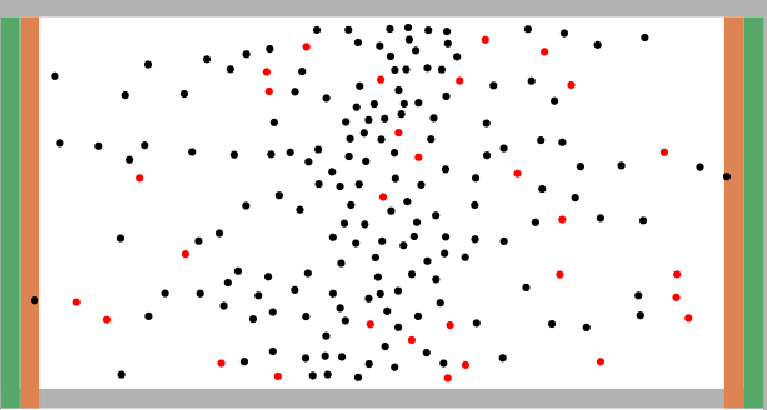
\includegraphics[width=0.4\textwidth]{report-template/images/corridor_20_0.png}}
\subfigure[infection rate 0.0001 after meet]{
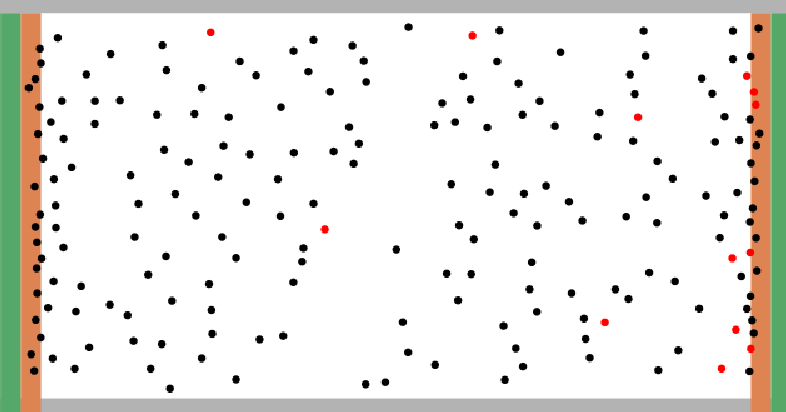
\includegraphics[width=0.4\textwidth]{report-template/images/0001_corridor_after_meet.png}}
\subfigure[infection rate 0.0001 at the end]{
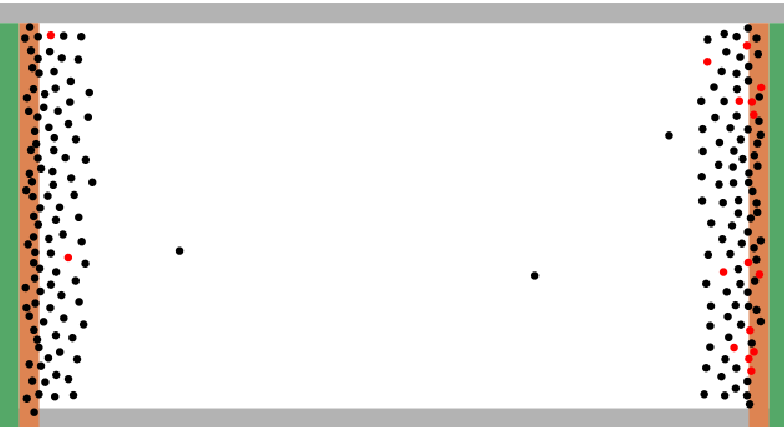
\includegraphics[width=0.4\textwidth]{report-template/images/0001_corridor_end.png}}
\caption{The corridor scenario}
\label{fig:corridor}
\end{figure}

\noindent Scenario \ref{fig:corridor}(a) parameters
\begin{verbatim}
"infectionsAtStart" : 10,
"infectionRate" : 1.0E-3,
"infectionMaxDistance" : 10.0,
"recoveryRate" : 0.0
"infectionRateWhenAdded" : 0.0
\end{verbatim}
Scenario \ref{fig:corridor}(b)(c) parameters
\begin{verbatim}
"infectionsAtStart" : 10,
"infectionRate" : 1.0E-4,
"infectionMaxDistance" : 10.0,
"recoveryRate" : 0.0
"infectionRateWhenAdded" : 0.0
\end{verbatim}


\paragraph{6. Decoupling infection rate from simulation time-step}
To do this we initially assume that an infected pedestrian has a chance of $(1-p)$ to not spread the disease. Let the probability of an infected pedestrian not spreading the disease at a \textit{single} time-step be $(1-q)$. Let $n$ be the amount of time-steps in a second, we then have the following equation:
\begin{align}
    (1-q)^n &=(1-p)\\
    (1-q) &= (1-p)^{1/n}
\end{align}
Note that the amount of time-steps $n$ in a second is equivalent to $n = 1/t$, where $t$ is the delta time or time since the last time-step has happened. Inserting this gives us the following:
\begin{align}
    (1-q) &= (1-p)^{1/(1/t)}\\
    (1-q) &= (1-p)^t
\end{align}
We have shown that that if a pedestrian does not spread the disease with probability $1-p$ every second, the chance to not spread the disease in delta time $t$ is $(1-q) = (1-p)^t$. Hence the chance that a pedestrian does spread the infection at a time-step is simply $1-(1-p)^t$.

To implement this we added an attribute \verb+LastSimulationTime+ to \verb+SIRGroupModel.java+, which is used to calculate the delta time $t$. In the \verb+update(...)+ function of the same class we then use the expression $1-(1-p)^t$ to correctly calculate the probability of infecting a pedestrian. Note that the same formula is used for recovery as well (See task 5.2).

The simulation rate still technically affects the infection. The infection radius and infection ticks caused by the new infected could be taken into account. For example if we instead simulated the infection retroactively. This however would necessitate ignoring simulation rate to an extent and therefore seems like a sub-optimal solution. If we truly wanted to allow the user to remove this inaccuracy at the cost of processing power it could be possible to add a separate simulation rate setting for the infection spread.



\paragraph{7. Possible extensions}
So far the integrated SIR model only contains basic features to model the spread of infections. Including the implementation from Task 5 the model would additionally consider the recovery of people. Still the SIR model as presented in \cite{boccara2010model} considers removed people instead of recovered people and therefore we only model infection in a simplified manner. In the following we will discuss possible extensions to improve the model.

The first possible extension is allowing recovered people to infect susceptible people. Recovered people realistically can still carry the infection around for a certain time. Therefore recovered people would still be able to infect susceptible people.

The second possible extensions is allowing recovered people to become reinfected. Simply speaking an infection could mutate within a group of people after a certain time frame. This mutated infection would then also be able to spread to recovered people and reinfect them.

Further more on completing the SIR model, under removed individuals we can consider subgroups other than recovered people. Here for example we could add deceased, permanently immune and/or isolated individuals. Disregarding the realism for a moment in the Vadere simulation this would mean deceased pedestrians could be modeled as static pedestrians. Permanently immune individuals would have 0 chance of being reinfected, where as isolated individuals are modeled as pedestrians performing social distancing.

At this point it becomes clear that the SIR model considers infection from a very general standpoint with the least amount of assumptions about the diverse factors that play a role in reality. The SIR model implemented in Vadere assumes that infections are spread by being in the vicinity of an infected pedestrian. This assumes that infections are spread through human interaction only. In Vadere we can extend this implementation to contain other groups that are carriers of infections. For example certain pedestrians could  be representing animals or insects. Similarly an infection that spreads through the air would could also be modeled as a group of infected pedestrians.

Beyond the assumption of modeling infections spreading in large crowds, we can also imitate the spread within social structures in Vadere. As shown in \cite{wolfram2020} an agent-based network provides an abstraction to model social connections. A majority pf people don't spend their time in crowds, but in certain environments with a set of other people e.g. workplace, school, university. This could be imitated in Vadere to a decently realistic degree. For example we can have the pedestrians form multiple smaller crowds at a sequence of targets and remain there for a certain time span. Here the targets can represent a home, workplace, school, supermarket, etc. A potential issue in this model would lie within the movement of the pedestrians between the targets. While infections do occur when traveling between different locations, this proposed model does not explicitly capture infections during traversal.

Overall we conclude this discussion with the fact that spread of infections in reality are very difficult to model due to a variety of factors. Every model is only an approximation of reality and depending on the assumptions made in the model, they provide a decently accurate depiction on certain aspects of it.

\end{task}